\documentclass[a4paper, 11pt]{article}
\setlength{\topmargin}{-0.5in}
\setlength{\textheight}{9.5in}
\setlength{\oddsidemargin}{-.1in}
\setlength{\textwidth}{6.5in}
\usepackage{graphicx}
\graphicspath{ {images/} }
\usepackage{datetime}

\newdateformat{monthyeardate}{%
  \monthname[\THEMONTH], \THEYEAR}

\date{}
\begin{document} 

\LARGE\title{Real Time Tempo Analysis of Drum Beats}

\LARGE\author{Author: \textbf{Philip Hannant}, Supervisor: \textbf{Professor Steve Maybank}\\
\\Birkbeck, University of London\\
Department of Computer Science and Information Systems\\
\\Project Proposal\\
MSc Computer Science\\
\\\monthyeardate\today
}





\normalsize


\maketitle
\newpage
\tableofcontents
\clearpage

\section*{Definitions}
\begin{tabular}{l p{4.5in}  }
\textbf{Acoustic Drum Kit} & A collection of drums and cymbals which do not have electronic amplification. Typically made up of a bass drum, snare drum, tom-toms, hi-hat and 1 or more cymbals.\\\\
% \textbf{Beat} & \\
\textbf{Downbeat} & The first beat of a piece of music.\\\\
\textbf{Drum Module} & The device which serves as a central processing unit an electronic drum kit, responsible for producing the sounds of the drum kit.\\\\
\textbf{Electronic Drum Kit} & An electrical device which is played like an acoustic drum kit, which produces sounds from a stored library of instruments and samples.\\\\
\textbf{MIDI} & Musical Instrument Digital Interface is a protocol developed in the 1980's which allows electronic instruments and other digital musical tools to communicate with each other [22].\\\\
\end{tabular}
\clearpage

\maketitle{} \section{Introduction and Background}
Having played the drums for nearly twenty years I have used a number of different training tools to help improve my timing. Until recently, these tools have always been exclusive to midi driven electronic drum kits, which are able to include training tools within their drum modules that use the events being triggered by the player to give live feedback on the exact timing and instrument being played. An example of such a system is the Roland DT-1 V-Drums tutor which is a software package that can be connected to a Roland V-Drum module in order to provide the player with an interactive experience that helps drummers improve their rhythm, coordination and sight reading [1]. Such an extensive and accurate range of tutoring functions is only made possible by the midi events that are intrinsic to an electronic drum kits function. (an example of the GUI can be found in figure 1). These tutoring tools are not however available to a drummer who does not own an electronic drum kit. Such a player is restricted to using a metronome and his/her ear to determine his/her timing and rhythm. To address this, I intend to investigate the accuracy of some of the available audio tempo analysis and beat tracking algorithms in order to ascertain which is more aligned to be implemented in drum tutoring software for acoustic drums.
\begin{figure}[h]
\caption{Example of Roland DT-1 V-Drums tutor GUI [1]}
	\centering
	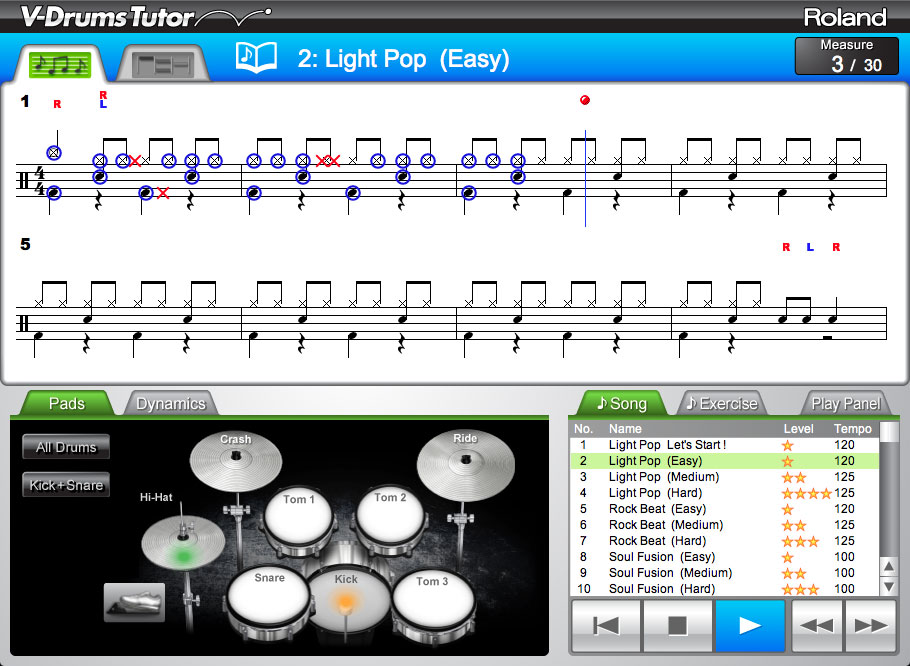
\includegraphics[scale=0.25]{dt-1_ss_main_notation_gal}
\end{figure}
\subsection{Beat Detection Background}

Detecting musical time is a skill which is not only fundamental to musicians [2] but also something that seemingly comes naturally to all humans. The majority are able to analyse and reproduce discrete metrical structures of a piece of music [3]. Longuet-Higgins [2] was one of the first to produce an algorithm to replicate this human ability, he constructed a binary tree with each node representing a note or rest [4]. He then developed his theory into a system that was able to react to how much the downbeats of a piece of music varied, which enabled the calculated tempo to be adjusted accordingly [2]. Since Longuet-Higgins' first work there have been a number of different approaches to beat detection in audio. M. Goto and Y. Muraoka created a system which learned the frequencies of the bass drum and snare drum, in order to detect events triggered by these instruments during a piece of music [5]. Simon Dixon [6] presented the system, Beatroot which processed a piece of audio generating a tempo hypotheses at various metrical levels. Multiple agents then find the sequence of beat times which best match the beats originally detected [6]. In the same year Tzanetakis, Essl and Cook [12] described an algorithm based on the Discrete Wavelet Transform which is capable of detecting the beat attributes of music. 

% Due to the rapidly expanding research being carried out on beat detection, the 1st annual Music Information Retrieval Evaluation eXchange (MIREX) was held in 2005. MIREX includes a contest with the goal of comparing state-of-the-art algorithms for music information retrieval [7]. The topics to be evaluated were proposed by the participants. In the first year, three of the nine topics concerned beat detection (Audio Drum Detection, Audio Onset Detection and Audio Tempo Extraction). 
To date, most beat detection software concentrates on static audio and is used extensively in the DJ industry where tempo and beat matching are popular functions. The software available for live tempo detection is limited to only a few live bpm detectors available in the App Store\footnote{Apple's application store - itunes.apple.com/uk/appstore‎} and Google Play\footnote{Google's application store for Android devices - play.google.com/store}. It is therefore a focus of this project to investigate if the beat detection system Beatroot and Tzanetakis, Essl and Cook's [12] method are accurate enough to be implemented in a live tempo drum beat analyser.

\subsection{Beatroot}
Beatroot is a Short-Time Fourier Transform based audio beat tracking system which is first presented by Simon Dixon in 2001 and is described as ``an off-line beat tracking system which finds the times of musical beats and tracks changes in tempo throughout a performance'' [13]. Beatroot works by first processing the audio data off-line to detect the rhythmic events and their relative timing, these events are then analysed and the possible tempo hypotheses are generated. Using the tempo hypotheses, multiple searches are carried out to find the sequence of beats which beat match the detected rhythmic events [27]. 

% \subsubsection{Onset Detection}
% Onset detection is a process used by most of beat detection methods currently available. The onset of a note is the instant which marks start of the variation in the frequency of a signal, a visualisation of this can be seen in figure 2. Once detected it can then be used to measure the onset times of sonic events\footnote{A sonic event is a singular feature of a piece music which can be made up of one source or many[24], e.g. the hitting of a drum} within a pieceof music [9].

% \begin{figure}[h]
% \caption{Visualisation of the onset within a signal [25]}
% 	\centering
% 	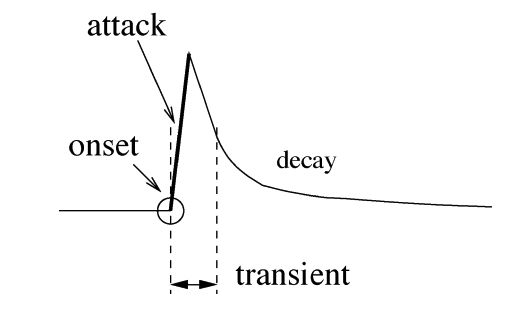
\includegraphics[scale=0.40]{Onset}
% \end{figure}

\subsubsection{Short-Time Fourier Transform}
The Short-Time Fourier Transform (STFT) is based on the original Fourier transform (FT) which was developed by Joseph Fourier in 1822. The Fourier transform can be used to find out how much of each frequency exists in a signal, a negative of the FT is that it is unable to provide any details of when a frequency component occurs in time for non-stationary signals\footnote{Non-stationary signals are signals whose frequency contents changes over time [10].}. A solution to this was to split a non-stationary signal up into a number of smaller segments using a window function, which effectively created a series of stationary\footnote{The frequency contents of a stationary signal does not change over time} signals which the original Fourier transform could then be successfully applied to. This however did not fully solve the problem as the size of window function affects the quality of frequency resolution and time resolution:
\begin{itemize}
\item Narrow Window Function $\longrightarrow$  Good Time Resolution, Bad Frequency Resolution
\item Wide Window Function $\longrightarrow$  Bad Time Resolution, Good Frequency Resolution [10]
\end{itemize}

\subsection{Tempo Analysis using the Discrete Wavelet Transform}
In 2001 Tzanetakis, Essl and Cook described how the Discrete Wavelet Transform (DWT) could be used to extract information from non-speech audio [12]. Their beat detection algorithm was based on detecting the most prominent signals which are repeated over a period of time within the analysed audio. The algorithm itself was split into the following steps: 

\begin{enumerate}
\item Signal decomposed into a number of octave frequency bands using the DWT
\item The subsequent time domain amplitude envelope is extracted for each frequency band, using low pass filtering, full wave rectification and downsampling
\item The envelopes of each band are then summed together and an autocorrelation function is computed
\end{enumerate}

There is no current open source Java implementation of this algorithm, however there is a Matlab implementation which has been created by Eng Eder de Souza [20]. This will form the basis for the DWT based beat detection component of this project.


\subsubsection{Discrete Wavelet Transform}
The first literature regarding the wavelet was provided by the mathematician Albert Haar in 1909 [26]. The wavelet transform is a technique for analysing signals which was developed as an alternative to the STFT [12]. Like the STFT the Discrete Wavelet Transform is able to provide time and frequency information, however unlike the STFT it is able to do this without a window function. The DWT's ability to provide high time and low frequency resolution for high frequencies and low time and high frequency resolution for low frequencies is considered to be similar to the time-frequency resolution characteristics demonstrated by the human ear [12].

\maketitle{}
\section{Aims and Objectives}
As part of my project I propose to build a real time drumbeat tempo analyser. This will use the Beatroot system described previously and an implementation of the Tzanetkis, Essl and Cook's beat detection algorithm [12] as a basis for the creation of a live drumming tempo training tool. I will elaborate on the key features of this work in the following sections.


\subsection{Core Project Features}
\begin{itemize}
\item Live audio capturing and processing
\item Adapt the Eng Eder de Souza Matlab implementation of the beat detection algorithm described by Tzanentkis, Essl and Cook [12] 
\item Build a system to record detailed comparative information regarding the efficiency and accuracy of Beatroot and Tzanetkis, Essl and Cook's algorithm in order to ascertain if they are accurate enough to be used in a training tool for drummers.
\item GUI which provides the current tempo played and beat detection
\item Although this is not a feature of the system, an extensive sample set of drum beats will need to be created to ensure the system is tested sufficiently.
\end{itemize}

\subsection{Non-Core Project Features}
\begin{itemize}
\item Investigate if it is possible for the system to learn the frequencies of the different drums being played
\item Extend GUI to provide the user with real time notification on when a certain drum is played
\end{itemize}

\maketitle{} 
\section{Development Plan for the Solution}

The main part of this project involves building a beat detection system in order to provide temporal analysis of a live audio signal. To do this I will use the Short-Time Fourier Transform based Beatroot and the algorithm described by Tzanetkis in [12] which will require the use of open source library JWave for the Discrete Wavelet Transform. 

\subsection{Live Audio Processing}
In order to capture and process live audio the Javax Sound package will be utilised, the audio will be captured in stereo and processed to match CD quality. This will be accomplished by using the Javax Sound AudioFormat class which will be constructed as follows:

\begin{itemize}
\item Encoding - This will be set to ``PCM.signed'', representing audio encoded to the native linear pulse code modulation, where quantization levels are linearly uniform [15].
\item Sample Rate - 44,100, set to match CD quality for the number of analog samples which will be analysed per second. 
\item Sample Size in Bits - 24, based on a sound card with a 24 bit sample depth.
\item Channels - 2, audio will be captured using a stereo microphone.
\item Frame Size - 6, where the frame size is the number of bytes in a sample multiplied by the number of channels [17].
\item Frame Rate - 44,100, same as sample rate.
\item Big Endian (boolean) - false, as the project will be developed on an Intel core which uses a little-endian architecture\footnote{Endianess refers to the order of bytes which make up a digital word. Big endianess stores the most significant byte at a certain memory address and the remaining bytes being stored in the following higher memory addresses. The little-endian formate reverses the order storing the least significant at the lowest and most significant at the highest memory address [16].}.
\end{itemize}

\subsection{JWave}
The implementation of Tzanentkis, Essl and Cook's [12] beat detection algorithm by Eng Eder de Souza used Matlab's inbuilt DWT functionality. To replicate this in Java, JWave will be used. JWave is a Java library created by Christian Scheiblich which provides a number different transform packages, including a wavelet package. For the purpose of this project the Daubechies wavelets classes within JWave will be used. The Daubechies wavelets are a form of discrete wavelet transform which were developed by ingrid Daubechies in the late 1980's and are frequently used in applications [27]. 

\subsection{Comparative Analysis of Beatroot and JWave}
A key part of this project is to ascertain whether the two beat detection methods described in section 1 are accurate enough to create a training tool similar to the midi based software seen in figure 1. To achieve this the two systems will need to be run in parallel using the same captured audio and return details on the calculated tempo in beats per minute (bpm), the number of beats detected and the time is took to calculate the results. 
% The tempo will be the beats per minute (bpm) recorded at the end of each processed frame, all of the bpm's within the sample set will be exact and in order to match the current midi software packages accuracy any returned bpm's should be exact as well. However, very small deviations in tempo can be very hard to detect to the human ear so some margin of error will be applied. To account for the fact that at the slower bpm's any beat out of place will be a lot easier to hear than at a higher bpm, the margin for error will be weighted by using the following equation;

% \[ m = (bpm - 60) * 0.0001\]
% \begin{flushleft}
% where \(m\) represents the weighted value for the margin for error to be applied.
% \end{flushleft}
The data collected during this process will be recorded and stored in an appropriate format to allow it to be queried and analysed. Due to the relatively small amount of data which will be collected it seems excessive to create a database to do this. Instead the data will be stored in a JSON file. JSON was chosen over XML as it has a much simpler grammar and is able to map directly onto the data structures used in modern programming languages [21].

\subsection{Build Extensive Drum Sample Set}
The success of this project will rely heavily on the amount of data that the system produces. A large set of drum beat samples will need to be created. The drum beats will be created using the Apple software package, Garageband. The sample set will contain beats from a variety of styles as well as samples with fluctuating tempos. The main aspects of the sample set are as follows:

\begin{itemize}
\item The tempo range will be 60 - 160 beats per minute. Some samples will be be created with varying tempos in order to model human playing more closely
\item The time signatures will be mainly in common time (4/4) to reflect normal playing styles, however some beats will use swing time which will either be created by feel\footnote{By adapting the strength a drum or cymbal is being played at it is possible to infer a different style of music using feel, e.g. swing time can be created this way.} within the sample or by using triplets with a duple meter in 12/8
\item Accenting, ghost notes and missed beats will be added in line with a real playing style
\item The sample set will contain a wide range of drum beats, including; beats using one drum, those only with a back beat, beats incorporating single rests within a bar or for the whole duration of a bar and beats with large solos and cymbal work
\end{itemize} 

Musical styles will comprise rock and pop, blues and jazz, with the main emphasis falling on rock and pop beats. Between 5 - 10 unique samples created for each style, which will be sampled with a range of bpms. Each sample will have approximately 20 different bpm values, accounting for approximately 500 separate samples. There will also be a final set of simple single and multiple drum beats included which will produce another c. 10 unique samples, which will result in a total sample set size of approximately 750 samples.

\subsection{Develop User Interface}
The user interface will be developed using the JavaFX framework, which will ensure that the system will be cross-platform compatible. Its features will be kept simple initially as it will only be required to display the current two tempo calculations and accumulative count of beats detected.

\subsection{Non-Core Project Features}
The non-core project features will be included only if the project is developed ahead of the schedule described in section 4. 

\subsubsection{Frequency Learning}
This additional feature will investigate if it is possible to recreate the system developed by Goto and Muraoka, which learnt the frequencies of the snare and kick drum in order to detect events triggered when these instruments were played [5]. The goal will be to enable the system to learn the frequencies of all of the separate parts of a drum kit (snare drum, bass drum, tom-tom, hi-hat and cymbals) being played and use this event to extend the GUI.

\subsubsection{Extended User Interface}
Developing this additional feature will only be possible if the previous non-core feature (3.6.1) is successfully developed. If so, the user interface will be extended to look similar to the drum kit visual seen in figure 1, where a colour indicator will be displayed to represent which instrument was last played. The development of this final feature depends heavily on the accuracy and efficiency of the tempo analysis algorithms used.

\subsection{Project Methodology}
This project will be developed using the Test Driven Development (TDD) framework. TDD is a development process that has very short development cycles. First a test is developed which is designed to fail, the minimum code is then written to pass this test and finally, the code is refactored accordingly to produce code at the appropriate standard [18].

\subsection{Development Languages and Testing}
The project will developed in a combination of Java and Scala. Java is required as both the Beatroot and JWave libraries are in this language, however any functional aspects of the project will be developed in Scala, as it offers a superior functional tool set when compared to those offered in Java 8. As previously discussed JSON will be used to store the collected data.

I will use the Intellij IDE to develop this system, Git will be used for version control and testing will be completed using JUnit for Java and Scala Test for any functionality developed in Scala. In order to ensure that the parsed JSON is well formed it will be tested using the JSON validator found at - http://jsonlint.com/.

\clearpage
\maketitle{} 
\section {Project Schedule}
The start date for the project is Monday 13th June 2016 and the end date is Monday 19th September 2016, the non-core project features will only be completed if the project is ahead of schedule.
\begin{table}[h]
\caption{Project Timeline} 
\centering
\begin{tabular}{|p{4cm}|p{8cm}|}
 \hline
\textbf{Dates} & \textbf{Task}\\ [0.5ex]
\hline 
w/c 13th June 2016 & Develop live audio capturing system\\
\hline 
w/c 20th June 2016 & Set up Beatroot library in development environment\\
\hline 
w/c 27th June 2016 & Implement DWT tempo and beat detection algorithm in Scala/Java\\
\hline 
w/c 4th July 2016 & Test systems with single live audio source\\
\hline 
w/c 11th July 2016 & Develop system to store data generated during tempo analysis\\
\hline 
w/c 18th July 2016 & Research and build appropriate framework to process captured audio in parallel e.g. akka actors\\
\hline 
w/c 1st August 2016 & Create sample set of drum beats\\
\hline 
w/c 8th August 2016 & Test system using full sample set\\
\hline 
w/c 15th August 2016 & Develop UI\\
\hline 
w/c 22nd August 2016 & Analyse logged data\\
\hline 
w/c 29th August 2026 & Write up report\\
\hline 
w/c 5th September 2016 & Present findings to project supervisor\\
\hline 
w/c 12th September 2016 & Finalise report\\
\hline 
w/c 19th September 2016 & Submit report\\
\hline
\end{tabular}
\end{table}
\clearpage
\maketitle{} 
\section{Summary}
I propose to build a real-time drumbeat tempo analysis system using the Short-Time Fourier Transform based Beatroot library and an implementation of the Tzanetkis et al [12] beat detection algorithm. An extensive set of drum samples will then processed through the system as live audio and the results recorded. These results will then be analysed to determine if the two beat detection methods are suitable to be implemented in a real time training tool for drummers.


\maketitle{} 
\section{References}
\begin{enumerate}
\item http://www.roland.co.uk/blog/exploring-roland-dt-1-v-drums-tutor-software/ %1
\item Allen and Dannenberg (1990), Tracking Musical Beats in Real Time, International Computer Music Conference, International Computer Music Association, pp. 140-143 %2
\item P. Desain and H. Honing (1989), The Quantization of Musical Time: A Connectionist Approach, Computer Music Journal, Vol. 13 No. 3 (Autumn), pp. 56-66 %3
\item H. C Longuet-Higgins (1976), Perception of melodies, Nature Vol. 263, pp. 646-653 %4
\item M. Goto and Y. Muraoka (1994), A beat tracking system for acoustic signals of music, in Proceedings of the Second ACM International Conference on Multimedia, pp. 365-372 %5
\item S. Dixon (2001), Automatic Extraction of Tempo and Beat from Expressive Performances, Journal of New Music Research, 30 (1), pp. 39-58. %6
\item http://www.music-ir.org/mirex/wiki/2005:Main\_Page %7
\item https://en.wikipedia.org/wiki/Onset\_(audio) %8
\item http://www.music-ir.org/mirex/wiki/2016:Audio\_Onset\_Detection %9
\item http://users.rowan.edu/~polikar/WAVELETS/WTpart2.html %10 
\item http://users.rowan.edu/~polikar/WAVELETS/WTpart4.html %11
\item G. Tzanetakis, G. Essl and P. Cook (2001), Audio Analysis using the Discrete Wavelet Transform, Proc. WSES International Conference on Acoustics and Music: Theory and Applications (AMTA) %12
\item S. Dixon (2003), On the Analysis of Musical Expression in Audio Signals, Storage and Retrieval for Media Databases, SPIE-IS\&T Electronic Imaging, SPIE Vol. 5021, pp. 122-132 %13
\item https://en.wikipedia.org/wiki/Discrete\_wavelet\_transform %14
\item https://en.wikipedia.org/wiki/Pulse-code\_modulation %15
\item https://en.wikipedia.org/wiki/Endianness %16
\item http://www.jsresources.org/faq\_audio.html %17
\item https://en.wikipedia.org/wiki/Test-driven\_development %18
\item A. Robertson, A. Stark and M. E. P. Davies (2013), Percussive Beat tracking using real-time median filtering, 6th International Workshop on Machine Learning and Music %19
\item https://github.com/ederwander/Beat-Track %20
\item http://www.json.org/xml.html %21
\item http://www.instructables.com/id/What-is-MIDI/ %22
\item http://disp.ee.ntu.edu.tw/tutorial/WaveletTutorial.pdf %23
\item http://www.ieor.berkeley.edu/~ieor170/sp15/files/Intro-to\_Sonic\_Events\_Campion.pdf %24
\item http://www.nyu.edu/classes/bello/MIR\_files/2005\_BelloEtAl\_IEEE\_TSALP.pdf %25
\item Gao, Robert X, Yan, Ruqiang (2011), Wavelets, Theory and Applications for Manufacturing %26
\item Andreas de Vries (2006), Wavelets %27
\item Simon Dixon (2001), An Interactive Beat Tracking and Visualisation System
\end{enumerate}
\end{document}
